%!TEX root = root.tex

\chapter{CHASMplus: enhanced context reveals the scope of somatic missense drivers in human cancers}
\label{chap:ch6}
\chaptermark{CHASMplus}

\section{Introduction}
In previous chapters, I have shown large-scale sequencing studies of patient cohorts have enabled identification of many genes or regions that when mutated \textit{can} act as cancer drivers. However, not every mutation in a driver gene or region is necessarily a driver of cancer; thus, requiring methods to discriminate whether an individual mutation is a driver or passenger.

The most common approach has been to apply machine learning to predict the cancer driver status of individual missense mutations by leveraging features characterizing a mutation, e.g., inter-species evolutionary conservation, features of the local protein environment, molecular function annotations, and biophysical characterizations of the amino acid substitution. Cancer-focused machine learning methods have previously tried to enhance performance by training cancer type specific models \cite{RN36, RN29} or boosting data with synthetic passenger missense mutations \cite{RN29}.  Unfortunately, a recent systematic study comparing 15 such methods concluded that none of them were sufficiently reliable for experimental or clinical follow-through \cite{RN134, RN136}. I and others have hypothesized that determining the impact of missense mutations requires proper context \cite{RN47}, which has not been sufficiently leveraged in a comprehensive manner in the current generation of methods. Context includes both prior knowledge about the functional importance of genes or gene subregions in which a mutation occurs, and mutational patterns that are now evident from cancer sequencing studies of many thousands of patients.

In this chapter, I present a new driver missense mutation prediction method, CHASMplus, that uses machine learning to integrate missense mutation context at multiple scales. The new CHASMplus consistently outperforms comparable methods, including the original CHASM, on eight different benchmark sets -- including in vitro experiments, in vivo experiments and literature benchmarks. Encouraged by these results, I applied CHASMplus to 8,657 The Cancer Genome Atlas (TCGA) samples from 32 cancer types to systematically identify driver missense mutations.

\section{CHASMplus algorithm}

\subsection{Overview}
CHASMplus uses the Random Forest algorithm to discriminate somatic missense mutations (referred to hereafter as missense mutations) that are drivers of human cancers from passenger missense mutations. A Random Forest is an ensemble of many randomized decision trees (see \autoref{chap:ch3}) \cite{RN41, RN40}. Each tree is trained on a random selection of training set examples and candidate features, via a recursive splitting process \cite{RN89}(\autoref{fig:chasmplus_overview}A). CHASMplus is trained using somatic mutation calls from The Cancer Genome Atlas (TCGA) covering 8,657 samples in 32 cancer types.  Because there is no gold standard set of driver and passenger missense mutations, I developed a semi-supervised approach to assign class labels to missense mutations, taking advantage of Random Forest robustness to noisy class labels.  Briefly, class labels are assigned so as to enrich the positive class for driver missense mutations (\autoref{fig:chasmplus_overview}B). CHASMplus training is done with a rigorous gene holdout cross-validation protocol to avoid overfitting, by ensuring all mutations within a gene are within the same fold \cite{RN128, RN137}. Therefore, missense mutations are never scored by a Random Forest trained on any missense mutation harbored by the same gene.  Finally, predicted scores from CHASMplus are weighted by the 20/20+ driver gene score, producing gene-weighted (gwCHASMplus) scores (\autoref{fig:chasmplus_overview}B).

\begin{figure}
  \centering
  \makeatletter
  \let\@currsize\normalsize
  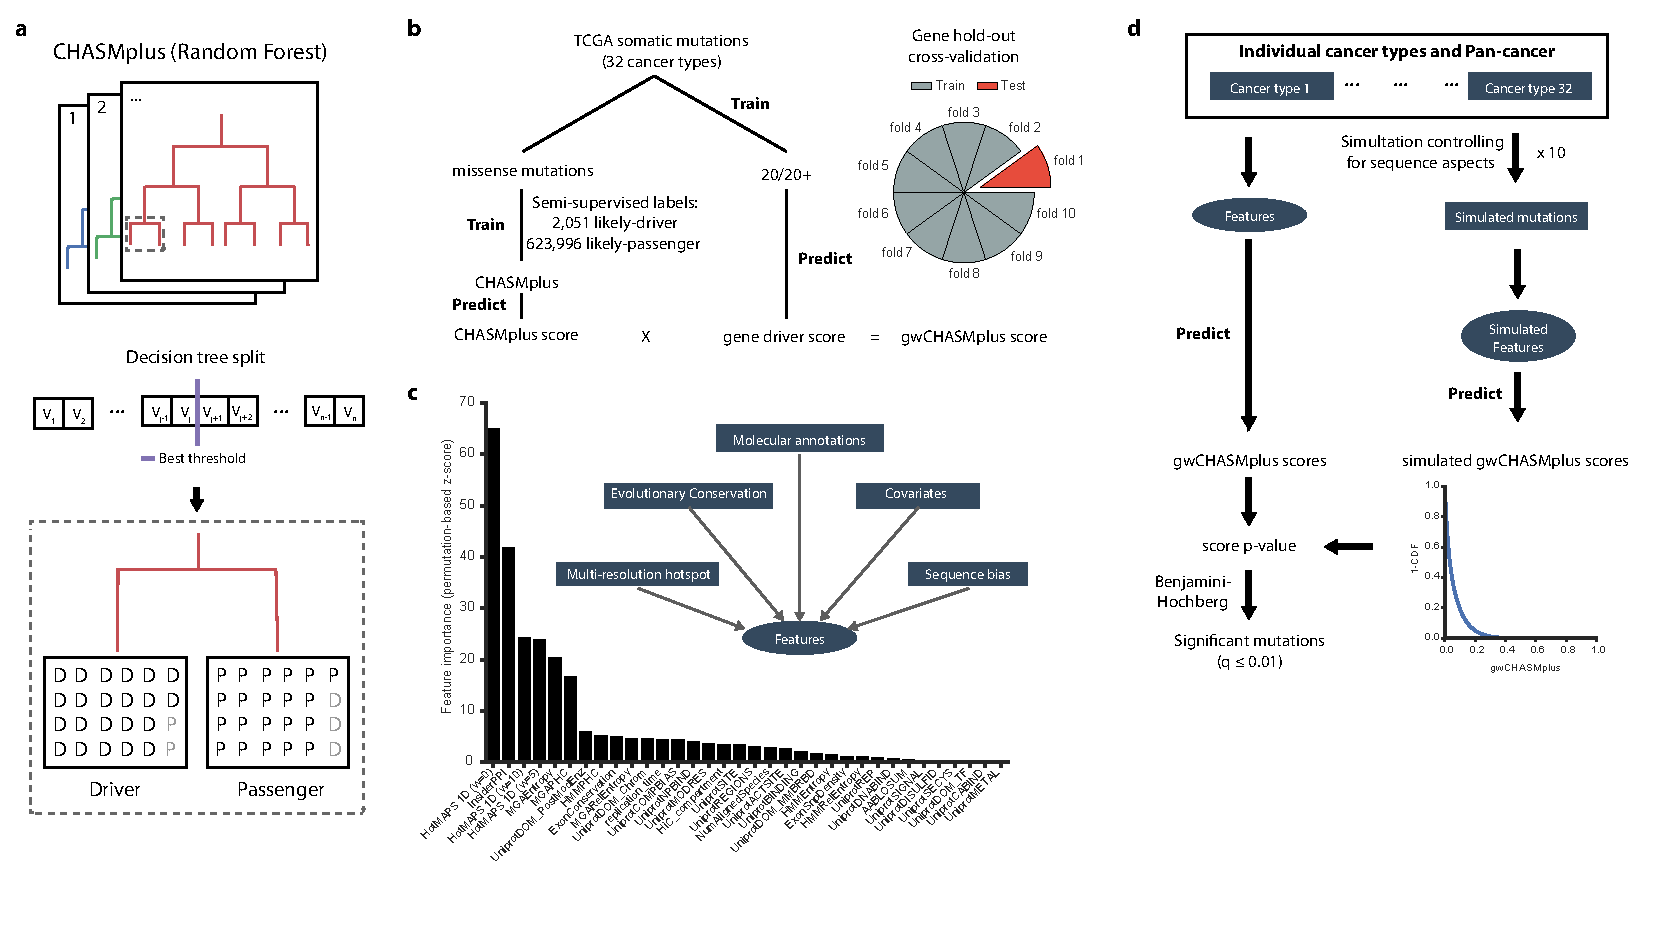
\includegraphics[width=\linewidth]{figures/chapter6/chasmplus_overview.pdf}
  \caption[Overview of CHASMplus algorithm.]{Overview of CHASMplus algorithm. a) CHASMplus predicts driver somatic missense mutations by using a random forest algorithm, consisting of an ensemble of decision trees. Each decision tree is constructed by selecting a random set of examples and features and recursively splitting examples by the best split criterion. b) Diagram of training and testing procedure by CHASMplus. c) Features with a net-positive feature importance by CHASMplus according to a permutation adjusted z-score. Boxed text indicates broad feature categories that were important. d) Diagram of how CHASMplus identifies statistically significant driver somatic missense mutations in each of the 32 cancer types individually and in aggregate (pan-cancer).}
  \label{fig:chasmplus_overview}
\end{figure}

\subsection{Semi-supervised training labels}
Using the TCGA mutation dataset, I established training labels with a semi-supervised approach, designed to minimize bias (\autoref{fig:chasmplus_flow_diagram}A). The positive class (likely-driver missense mutations) was selected by the following criteria: 1) missense mutations had to occur in a curated set of 125 pan-cancer driver genes \cite{RN25}; 2) for each of the 32 TCGA cancer types, missense mutations found in that cancer type had to occur in a significantly mutated gene for that cancer type according to MutSigCV v1.4 \cite{RN14}. I ran MutSigCV using recommended settings and a full sequencing coverage file (\url{http://archive.broadinstitute.org/cancer/cga/mutsig}).  Importantly, MutSigCV v1.4 only assess the total number of mutations in a gene, and not any characteristics of those mutations; thus, I avoid making strong assumptions about the properties of a particular driver mutation; 3) missense mutations had to occur in samples with relatively low mutation rate (less than 500 mutations, half the minimum hypermutator threshold).  This filter was intended to limit the number of passenger mutations mislabeled as drivers.  The negative class (likely-passenger missense mutations) consisted of the remaining missense mutations in the TCGA mutation set.  For training purposes, I only used unique mutations to avoid double counting a mutation seen more than once. If, however, the same mutation consequence observed in different cancer types had contradictory labels, I regarded the mutation as a driver because mutation recurrence is often cited as supportive evidence for a cancer driver role. This established a set of 2,051 likely-driver missense mutations and 623,996 likely-passenger missense mutations, for which I found sufficient annotation to compute our selected features.

\begin{figure}
  \centering
  \makeatletter
  \let\@currsize\normalsize
  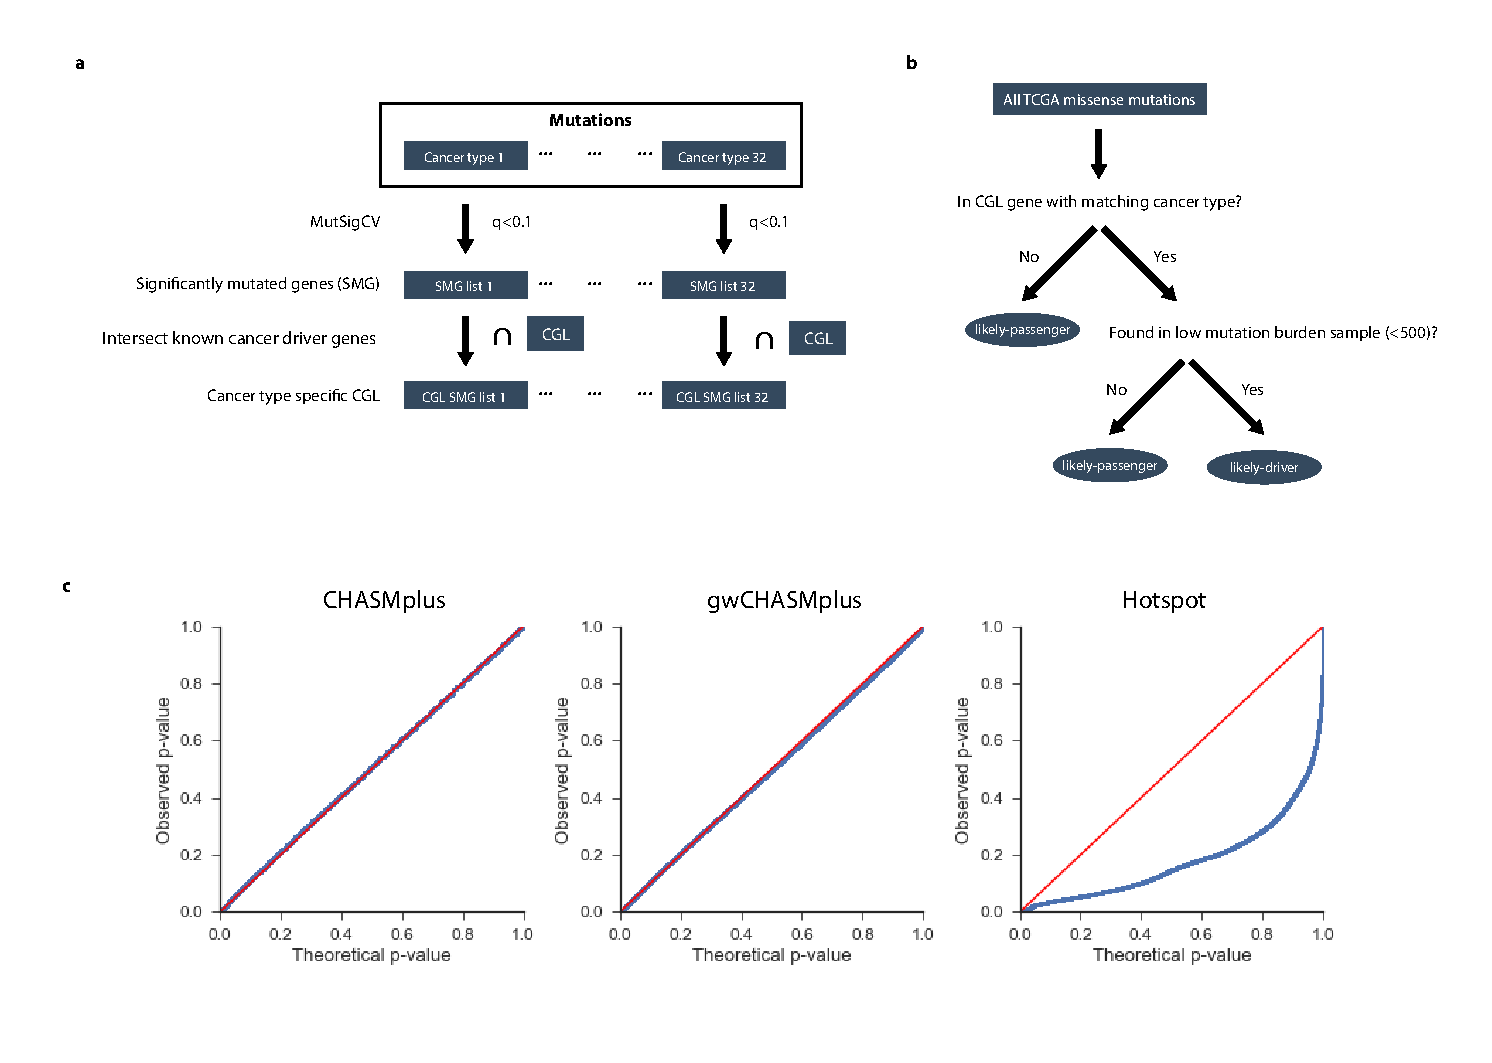
\includegraphics[width=\linewidth]{figures/chapter6/chasmplus_flow_diagram.pdf}
  \caption[Training set labeling procedure and calibration of statistical model]{Training set labeling procedure and calibration of statistical model. a) Diagram demonstrating how the cancer type specificity of Cancer Genome Landscape (CGL) genes were determined. b) Somatic missense mutations were labeled either as \q{likely-passenger} or \q{likely-driver} based on a semi-supervised approach using two steps: overlap with previously known genes from CGL in a cancer type specific manner and samples with low mutation burden. c) QQ plot of observed p-values for a method (blue line) compared to theoretically expected under the null hypothesis (red line). All mutations in genes found in the Cancer Gene Census were removed to eliminate possible driver mutations in this comparison. CHASMplus represents unweighted CHASMplus scores, gwCHASMplus represents gene weighted CHASMplus scores, and Hotspot is a previous codon-level mutation hotspot detection method.}
  \label{fig:chasmplus_flow_diagram}
\end{figure}

\subsection{Features}
CHASMplus scores benefit from representation of missense mutation context at multiple scales. The Random Forest was trained on 95 features, and the 34 features with a net positive feature importance are shown in \autoref{fig:chasmplus_overview}C. Important features assess five broad categories: multi-resolution missense mutation hotspots (HotMAPS 1D algorithm \cite{RN60}), evolutionary conservation/human germline variation, molecular function annotations (e.g., protein-protein interface annotations from \cite{RN139}), sequence biased regions, and gene-level covariates (e.g., replication timing). Missense mutation context is further represented by the 20/20+ driver score of the gene harboring the missense mutation and the specific cancer type in which it was observed.  While gene-level features have been previously applied to missense mutation driver prediction \cite{RN35}, to my knowledge, this is the first time that gene-level and missense mutation-level driver scores have been coupled in a cancer type-specific manner.  

\subsection{Statistical significance}
CHASMplus can also evaluate the statistical significance of cancer type-sepcific predictions for each of 32 cancer types from The Cancer Genome Atlas (TCGA), and pan-cancer predictions for all TCGA cancer types in aggregate (\autoref{fig:chasmplus_overview}D). Because Random Forests do not intrinsically include hypothesis testing techniques, I used simulated mutations to assess the statistical significance of scores. P-values were estimated from a simulated null distribution, controlling for sequence composition, and corrected for multiple testing with the Benjamini-Hochberg method (see \autoref{sec:monte_carlo}). The resulting P-value distributions suggest our statistical model is well calibrated (\autoref{fig:chasmplus_flow_diagram}B).  Well-calibrated P-values enable quantitative estimates of false discovery rate and thus inform a user about how to select a suitable score threshold for predicted driver missense mutations.

\section{CHASMplus dramatically improves identification of  missense mutation drivers}
I next sought to compare the performance of CHASMplus on seven mutation-level benchmarks with respect to 12 comparable methods: VEST \cite{RN30}, CADD \cite{RN34}, FATHMM cancer \cite{RN39}, SIFT \cite{RN116}, MutationAssessor \cite{RN38}, REVEL \cite{RN32}, MCAP \cite{RN33}, ParsSNP \cite{RN35}, CHASM \cite{RN29}, Polyphen2 \cite{RN28}, transFIC \cite{RN31} and CanDrA \cite{RN36}. Scores were obtained by means made available by each of the methods. 

My benchmarks fall under three broad categories: in vitro experiments, high throughput in vivo screens, and curation from published literature.  Each of these categories has weaknesses, but, in aggregate, they span multiple scales of evaluation and amount of supportive evidence (\autoref{fig:chasmplus_benchmark}A). For example, several benchmarks are limited to one or a few well-established driver genes, while others are exome-wide, but lack experimental support. A range of benchmarks is critical because missense mutations with the most established experimental support for a driver role tend to be in a few well-understood cancer driver genes.  However, limiting benchmarking to these genes makes it difficult to assess the generalizability of a method's performance to missense mutations in other genes. All benchmark evaluations used the area under the Receiver Operating Characteristic Curve (auROC) as a metric (\autoref{fig:chasmplus_benchmark}B).  Overall, CHASMplus had a mean auROC of 0.09 higher than the next best method. This common metric is used in machine learning to describe how well predictions separate two classes without a priori selecting a score threshold, which for many methods is not well defined \cite{RN140}. In our assessment, the two classes represent likely driver and passenger missense mutations. In general, auROC values range from 0.5 (random prediction performance) to 1.0 (perfect).

\begin{figure}
  \centering
  \makeatletter
  \let\@currsize\normalsize
  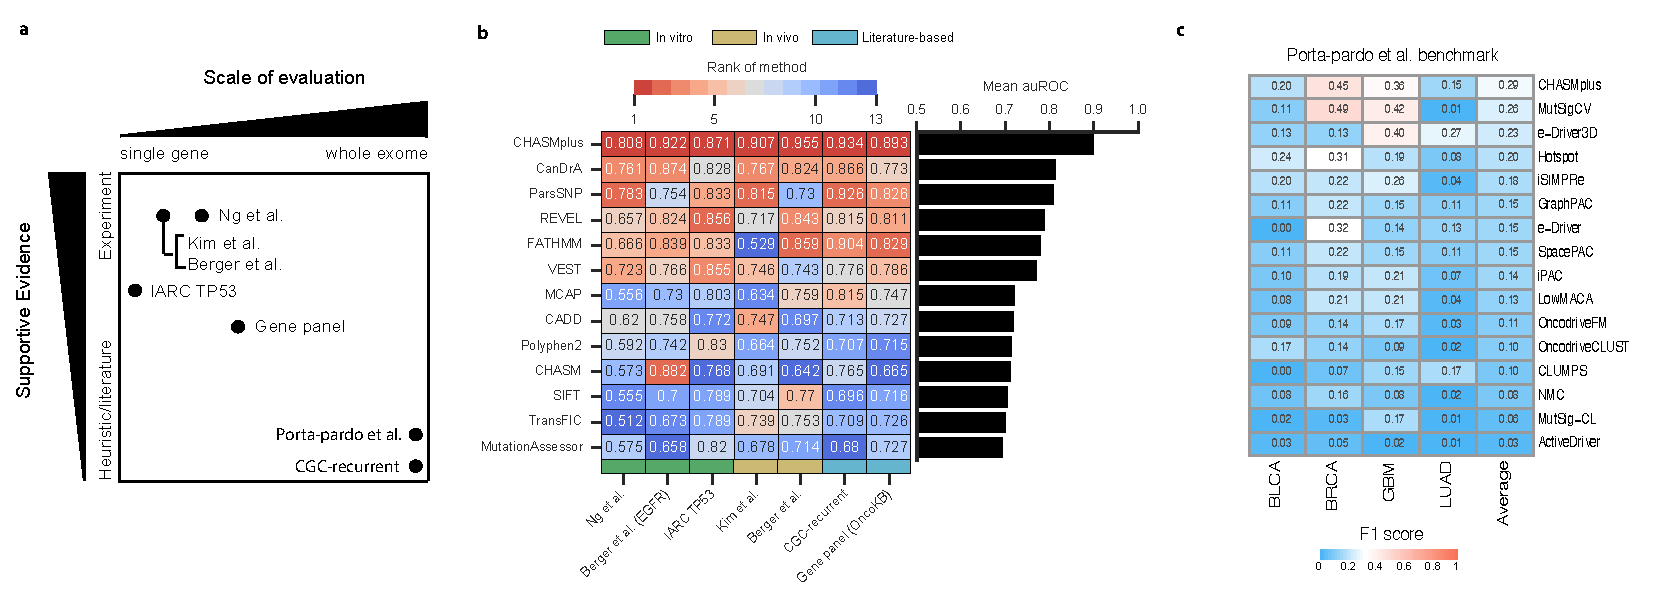
\includegraphics[width=0.9\linewidth]{figures/chapter6/chasmplus_benchmark.pdf}
  \caption[Cancer driver prediction benchmark.]{Cancer driver prediction benchmark. a) Conceptual diagram of how 8 benchmarks compare in terms of the scale of evaluation and amount of supportive evidence. b) A heatmap showing performance measured by the area under the Receiver Operating Characteristic Curve (auROC) on the 7 mutation-level benchmarks (shown in text). The color scale from red to blue indicates methods ranked from high to low performance.  Benchmarks are categorized by in vitro (green), in vivo (yellow), and literature-based benchmarks (turquoise). The bar graph shows the mean auROC across the benchmarks. c) Heatmap showing performance (F1 score) on a cancer type specific benchmark. The overall performance on four cancer types (BLCA, BRCA, GBM, and LUAD) is measured by the average F1 score (right column).}
  \label{fig:chasmplus_benchmark}
\end{figure}

I used three benchmarks based on in vitro experiments. The first was a set of missense mutations assessed by an assay of cell viability in two growth-factor dependent cell lines, Ba/F3 and MCF10A (pro-B and breast epithelium cell lines), covering 747 mutations in 48 genes \cite{RN187}. CHASMplus had significantly higher performance than the next best performing method (ParsSNP) (p$<$0.05, delong test). In the second benchmark, an in vitro assay of EGFR resistance to erlotinib from missense mutations observed in lung adenocarcinoma \cite{RN141}, CHASMplus (auROC=0.92) outperformed all other methods, with the next best method (CanDrA) having an auROC of 0.87.  CHASMplus auROC was significantly better than that of 7 of the methods tested (p$<$.05, delong test).  For the remaining 5 methods, the improvement was not significant, possibly due to lack of power given the small number of mutations (n=75) tested in the assay.  In the third benchmark, an assay of reduced transactivation ($<$50\% WT, median of 8 targets) in TP53 from the IARC database (n=2,314 mutations)\cite{RN142}, CHASMplus significantly outperformed the next best method (REVEL) (p=0.02, delong test).

To investigate whether CHASMplus would also perform well when compared to results of in vivo experiments, I considered two benchmarks based on pooled in vivo screens in mice that assessed mutation driver status by fitness in a competition assay.  The first was performed from mutations observed in lung cancers (44 missense mutations) \cite{RN141} and the second from mutations observed in 27 cancer types (71 missense mutations) \cite{RN143}. CHASMplus had the highest auROC of the 13 tested methods on both benchmarks, with an increase in auROC by 0.09 and 0.1, respectively, compared to the next best methods (ParsSNP in the first benchmark and FATHMM in the second). The increase was significant in the second larger, benchmark (p=0.03, delong test, n=72), but not in the first, which may be the result of the smaller sample size.  In the first benchmark, CHASMplus was significantly better than 9 out of 12 tested methods (p$<$0.05, delong test, n=44).

Experimental testing of mutations across large number of genes or the whole exome is currently not feasible. Therefore, evaluation of CHASMplus at larger scales relied on two benchmarks based on literature and database curation. The first benchmark in this category labeled recurrent missense mutations within genes in the Cancer Gene Census \cite{RN97} as drivers. I found that the gene weighted CHASMplus scores (auROC=0.934) were substantially better at this whole exome-wide prioritization task compared to the unweighted CHASMplus scores (auROC=0.893) (p$<$2.2e-16, delong test). CHASMplus scores were also significantly better than the next best method (ParsSNP) (p=0.001, delong test). The second benchmark was derived from a large driver gene panel (MSK-IMPACT, 414 genes) and 10,130 sequenced cancer patients \cite{RN145}.  Missense mutations were labeled as drivers if they were annotated as such in OncoKB \cite{RN144}, a knowledge-base that aggregates known literature. CHASMplus significantly outperformed all other methods, the nearest being ParsSNP (p=7e-14, delong test). 

\section{CHASMplus improves identification of cancer type specific driver genes}
I evaluated the performance of CHASMplus on identifying cancer-type specific driver genes, using a previously published benchmark and assessment of 15 computational methods designed for this purpose \cite{RN52}. The 15 methods are: Hotspot \cite{RN16}, NMC \cite{RN106}, OncodriveCLUST \cite{RN54}, MutSig-CL \cite{RN14}, iSiMPRe \cite{RN150}, iPAC \cite{RN15}, GraphPAC \cite{RN151}, SpacePAC \cite{RN152}, CLUMPS \cite{RN105}, e-Driver \cite{RN153}, e-Driver3D \cite{RN45}, ActiveDriver \cite{RN154}, LowMACA \cite{RN155}, OncodriveFM \cite{RN53}, and MutSigCV \cite{RN13}. Genes were labeled by their designations in the Cancer Gene Census as a cancer driver gene for a specific cancer type. Out of the 4 cancer type cohorts assessed (BLCA, BRCA, GBM, and LUAD), CHASMplus had the highest average F1 score, a balance between precision and recall that was used as a performance metric by \cite{RN52} (\autoref{fig:chasmplus_benchmark}C). I additionally note that of the methods tested, CHASMplus was the only one not primarily designed to predict driver genes that had high recall (average recall=.45) while maintaining precision (average precision=.23). 

\section{CHASMplus identified both common and rare cancer drivers}

Certain cancer driver mutations primarily occur in a specific cancer type, while others appear in many cancer types.  The power to detect driver mutations, which occur at low frequency in many cancer types, is increased when many cancer types are aggregated, known as a pan-cancer analysis. Conversely, driver mutations, which are specific to a particular cancer type, are best identified when cancer types are analyzed individually \cite{RN59}. Using CHASMplus, I identified 3,527 unique missense mutations as statistically significant drivers by pan-cancer analysis at an estimated false discovery rate of 1\%. When applied to each cancer type individually, the number found significant varied substantially from 8 in thymoma to 572 in bladder urothelial carcinoma with a median of 78 (\autoref{fig:chasmplus_tcga}A). The median overlap with literature-based oncogenicity annotation from OncoKB was 53\%, suggesting 47\% of the driver missense mutations identified by CHASMplus either have not been previously characterized or not sufficiently characterized for inclusion in OncoKB.  While OncoKB missense mutation annotations are not cancer-type specific, the genes with highest frequencies of cancer-type specific driver missense mutations identified by CHASMplus have well-known roles in cancer \cite{RN5} (\autoref{fig:chasmplus_tcga}B). 

\begin{figure}
  \centering
  \makeatletter
  \let\@currsize\normalsize
  \includegraphics[width=0.9\linewidth]{figures/chapter6/chasmplus_tcga.pdf}
  \caption[Discovery of driver missense mutations by CHASMplus]{Discovery of driver missense mutations. a) Bar graphs showing the number of unique driver somatic missense mutations (top) and the proportion previously known in OncoKB, a literature curated database (bottom). b) Heatmap of the top 25 genes containing the most frequent driver somatic missense mutations in TCGA across the cancer type specific analyses. Shown are the percentage of samples that are mutated. c) Proportion of overall frequency of driver somatic missense mutations found in rare ($<$1\% of samples or singleton mutations), intermediate (1-5\%), and common ($>$5\%) driver somatic missense mutations. Correspondingly shown as light to dark blue. d) Structure of the Phosphatase 2A holoenzyme (PDB 2IAE). e) Structures of the ERBB2 extracellular domain (left, PDB 2A91) and kinase domain (right, PDB 3PP0).}
  \label{fig:chasmplus_tcga}
\end{figure}

The long tail hypothesis, proposed from examining overall mutation frequency of driver genes \cite{RN147, RN148}, suggests there are many rare drivers. However, the overall mutation frequency of a gene does not account for the confounding presence of passenger mutations within a driver gene. From our mutation-level analysis, I observed that the relative prevalence of rare ($<$1\% of samples), intermediate (1-5\%), and common ($>$5\%) driver missense mutations varied substantially among cancer types (\autoref{fig:chasmplus_tcga}C). For example, uveal melanoma was dominated by common driver missense mutations (88\%), while head and neck squamous cell carcinoma (HNSC) was dominated by rare driver missense mutations (63\%). Interestingly, from the pan-cancer analysis, the overall proportion of driver missense mutations considered rare was only slightly smaller than for common drivers (35.4\% and 35.5\%, respectively), but 4-fold greater than found by a previous method (8\%, P<2.2e-16, Fisher’s exact test) \cite{RN23}.

Rare driver missense mutations exist not only in rare driver genes, but also may be spatially proximal in protein structure to common driver missense mutations. For example, the protein phosphatase PPP2R1A, which has been implicated as a tumor suppressor gene in many tumor types \cite{RN57}, contained common driver missense mutations in our pan-cancer analysis at residue positions 179 and 183, which is located at the protein interface composing the phosphatase 2A complex (\autoref{fig:chasmplus_tcga}D). It also had a much broader set of rare drivers throughout the protein interface, such as R105Q and R459C.  Similarly, CHASMplus identified common driver missense mutations (S310A/F/Y) in the extracellular domain of the well-known oncogene ERBB2, but also finds rare driver missense mutations in both the extracellular and kinase domain (e.g., L313V and R678Q) (\autoref{fig:chasmplus_tcga}E). This is supportive of previous experimental work implicating rare cancer driver mutations in common cancer driver genes \cite{RN4}.

\section{Mutation hotspot detection has limited power}
A codon or small region of protein sequence or structure where recurrent mutations are observed is known as a hotspot.  Similar to statistical methods for driver gene detection, hotspot detection identifies an excess number of mutations compared to expectation. using a large number of cancer samples.  I asked whether, given current cohort sizes, codon-based hotspot detection had sufficient statistical power to identify rare driver mutations.  I assessed the number of samples required to detect driver mutations across a range of frequencies (proportion of samples in which a mutation occurs) and somatic background mutation rates. In \autoref{fig:chasmplus_power}A, each of the 32 TCGA cancer types is placed according to its sample size and background mutation rate, relative to six curves which represent the required sample size to detect driver mutations of a certain frequency, with 90\% power, using hotspot detection.  For example, the TCGA Cervical Squamous Cell Carcinoma and Endocervical Adenocarcinoma (CESC) cohort has 274 samples and a background mutation rate of 3.5 mutations/Mb.  This sample size is sufficient to detect driver mutations that occur in ~2\% of the samples with 90\% power. 

\begin{figure}[b!]
  \centering
  \makeatletter
  \let\@currsize\normalsize
  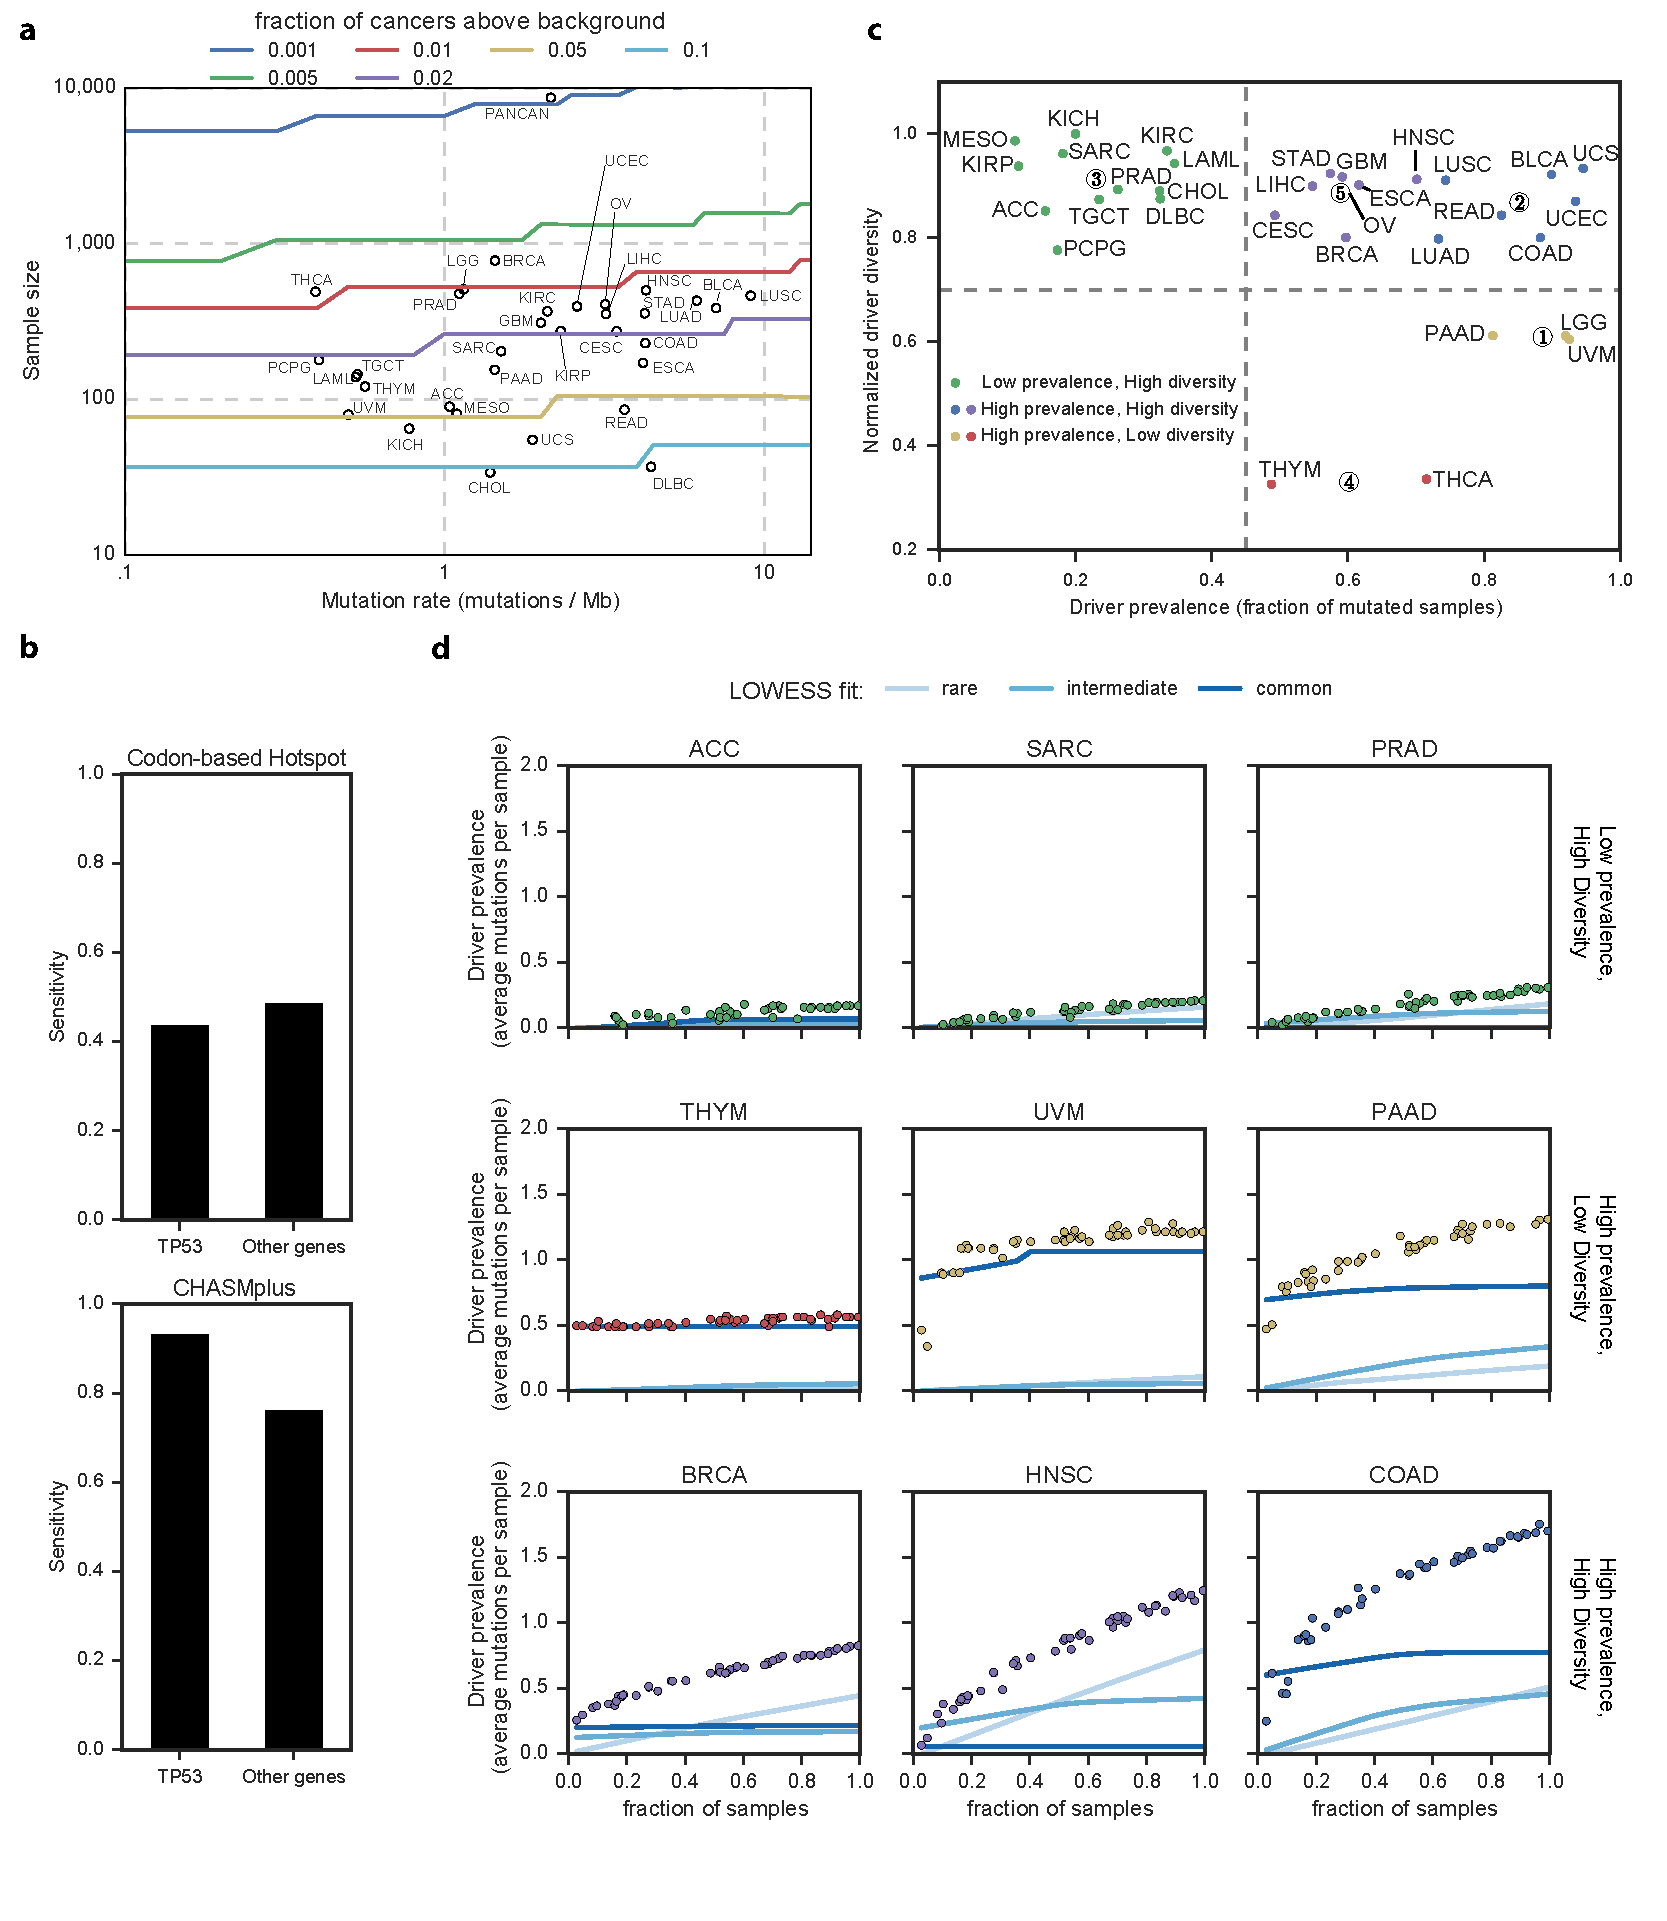
\includegraphics[width=\linewidth]{figures/chapter6/diversity_and_saturation.pdf}
  \caption[Saturation and characteristics of driver somatic missense mutations.]{(Caption next page.)}
  \label{fig:chasmplus_power}
\end{figure}
\addtocounter{figure}{-1}
\begin{figure} [t!]
  \caption[(continued) Saturation and characteristics of driver somatic missense mutations.]{(Figure: previous page) Saturation and characteristics of driver somatic missense mutations. a) Statistical power to detect significantly elevated non-silent mutations for individual codons as a function of sample size and mutation rate. Circles represent each cancer type from the TCGA, and is placed according to sample size and median mutation rate. Curves are colored by the effect size of the driver mutations (fraction of non-silent mutated cancer samples above the background mutation rate). b) Bar graph comparing sensitivity to detect labeled oncogenic driver missense mutations from OncoKB between CHASMplus and a hotspot detection approach. c) Plot displaying normalized driver diversity and driver prevalence (fraction of samples mutated) for driver somatic missense mutations in 32 cancer types. K-means clustering identified 5 clusters with centroids shown as numerically designated circles. d) Prevalence of driver somatic missense mutations as a function of sample size. Lines represent LOWESS fit to different rarities of driver somatic missense mutations.}
\end{figure}

At current TCGA sample sizes, I found codon-based hotspot detection approaches were not well powered to identify driver mutations that occurred at less than 1\% frequency in most cancer types.  Exceptions were thyroid carcinoma (THCA), low grade glioma (LGG) and breast cancer (BRCA), which are seen to lie above (or close to) the curve representing 1\% frequency (\autoref{fig:chasmplus_power}A).  Notably, these cohorts had large numbers of samples and low-to-medium background mutation rates.  I also found that when cancer types were aggregated in pan-cancer analysis, power to detect codon-based hotspots improved substantially, but only when the recurrent mutations were shared in more than one cancer type.  For these mutations, pan-cancer analysis using ~10,000 TCGA samples should enable detection of driver mutations at frequency as low as 0.1\%.   

In our pan-cancer analysis, CHASMplus had greater sensitivity to detect putatively oncogenic missense mutations than a recently published codon-based hotspot detection method (\autoref{fig:chasmplus_power}B). I compared the missense mutations in the TCGA pan-cancer cohort that were called statistically significant by CHASMplus and those called by a hotspot method described by \cite{RN23} ($q\leq 0.01$ for both methods).  For each method, I computed the overlap with well-curated oncogenic mutations in the OncoKB database.  CHASMplus sensitivity to detect the OncoKB-labeled mutations was 0.83.  The sensitivity of the hotspot method (0.46) was significantly lower (p$<$2.2e-16, McNemar's test, n=896).  To minimize gene bias, I also repeated the analysis after excluding all 389 TP53 mutations, yielding sensitivity of 0.76 for CHASMplus and 0.49 for hotspot detection, a difference which is still statistically significant (p<2.2e-16, McNemar's test, n=507). Moreover, these results are also reflected in the number of significant predictions of the two methods.  The codon-based hotspot method only identified 360 unique codons as significant in our TCGA data set, while CHASMplus found significant missense mutations in 2,588 codons. I believe that the increased sensitivity is the result of CHASMplus using a broad range of important features, including multi-resolution hotspot detection and weighting by driver gene scores (\autoref{fig:chasmplus_power}C).  Importantly, my increased sensitivity did not come at the cost of low specificity, as evidenced by our p-value calibration and extensive ROC analysis across seven benchmarked datasets, which measures a balance of sensitivity and specificity.

\section{Characterizing cancer types and the trajectory of discovery}
The diversity and prevalence of driver missense mutations varied considerably across TCGA cancer types (\autoref{fig:chasmplus_power}C).  I defined diversity with respect to the distribution of driver missense mutations across codons and prevalence with respect to the frequency of the mutations in tumor samples.  High diversity indicated mutations were broadly distributed across codons, while high prevalence indicated driver missense mutations that occurred in a large number of tumor samples. Using K-means clustering, I found that cancer types grouped into high diversity and low prevalence (12 cancer types), high diversity and high prevalence (15 cancer types), and low diversity and high prevalence (5 cancer types). These differences were not associated with intra-tumor heterogeneity or normal contamination, as assessed by mean variant allele fraction (VAF) of a cancer type (p$>$0.05, correlation test).  The differences also could not be associated only with TCGA sample size for a particular cancer type.  For example, while both pancreatic ductal adenocarcinoma (PAAD) and sarcoma (SARC) had similar sample sizes (n=155, n=204 respectively), PAAD had high prevalence and low diversity, while SARC had low prevalence and high diversity. After adjusting for sample size, I observed that the average mutation burden for a cancer type positively correlated with the prevalence of rare (but not common) driver missense mutations (R=0.63, P=4.7e-5, likelihood ratio test).

Are there substantially more cancer driver missense mutations yet to be discovered? If discovery was measured by the number of unique driver missense mutations identified, subsampling analysis showed all cancer types had a linear increase ($R^2>0.5$) with no evidence of saturation at current sample sizes (\autoref{fig:chasmplus_subsampling}).  However, I did observe substantial variability in trajectories if discovery was measured by driver prevalence (average number of driver missense mutations per cancer sample) (\autoref{fig:chasmplus_power}D), a metric which goes directly to utility of driver discovery in clinical practice (Discussion). For sarcoma (SARC), adrenocortical carcinoma (ACC), and prostate adenocarcinoma (PRAD), driver prevalence remained minimal as sample size increased.  While, in contrast, thymoma (THYM), uveal melanoma (UVM), and pancreatic ductal adenocarcinoma (PAAD) contained common driver missense mutations that could be detected by using only a few samples from the cohort, e.g., GTF2I L424H in THYM.  Due to a lack of rare or intermediate driver missense mutations, I observed THYM and UVM saturated discovery as sample size increased. Although PAAD did show a growing set of intermediate/rare driver missense mutations, the overall driver prevalence exhibited a diminishing rate of discovery. In contrast, breast (BRCA), head and neck squamous (HNSC), and colon cancers (COAD) harbored a full spectrum of driver missense mutations, with rare drivers increasing substantially as a function of sample size.

\begin{figure}
  \centering
  \makeatletter
  \let\@currsize\normalsize
  \includegraphics[width=0.9\linewidth]{figures/chapter6/sub_sampling_num_unique.pdf}
  \caption[Subsampling analysis of unique driver somatic missense mutations by CHASMplus.]{Subsampling analysis of unique driver somatic missense mutations by CHASMplus. The number of driver somatic missense mutations identified as significant by CHASMplus ($q \leq 0.01$) as a function of sample size. CHASMplus was ran on random subsets of various sizes (fraction of samples) of the full data.}
  \label{fig:chasmplus_subsampling}
\end{figure}

\section{Discussion}

CHASMplus was designed to better represent the context in which missense mutations occur, by coupling prior information about a mutation's likely functional importance and mutational patterns evident from large cancer sequencing studies. I compared CHASMplus with 27 other computational methods, including the original CHASM, on eight benchmarks covering in vivo experiments, in vitro experiments, and literature curation, CHASMplus had the best performance at predicting drivers at each scale of evaluation - a whole exome, a targeted gene panel, and within a single gene.   Individually, none of the benchmarks was ideal.  For example, mutations in the in vitro or in vivo benchmarks, were selected by complicated study inclusion criteria and limited by resource constraints.  However, I believe that application of multiple independent benchmarks spanning a wide array of genes is the current best practice.

The long tail hypothesis \cite{RN147, RN148} posits that there are many rare driver mutations in human cancers. To assess this hypothesis, I leveraged the improvements made in CHASMplus to systematically predict driver missense mutations in 8,657 samples from the TCGA. Although individually rare, I found that rare driver missense mutations played a prominent role in aggregate, consistent with the long tail hypothesis. This result supports the critical role of assessing the prevalence of driver mutations -- failure to capture and identify rare driver mutations, which occur in aggregate at reasonable prevalences, may result in crucial missed opportunities.   Because high-throughput functional validation studies of missense mutations are not yet widespread, computational methods, like CHASMplus, are needed to prioritize mutations for low- and medium-throughput studies. A key advantage of CHASMplus is that I can precompute a score for every possible missense mutation, forming an \textit{in silico} saturation mutagenesis across all genes to capture rare driver mutations yet seen mutated.

To my knowledge, mine is the first study to show that the prevalence and diversity of driver missense mutations is highly variable across the cancer types represented in the TCGA.  I observed that mutation burden for a cancer type positively correlated with prevalence of rare (but not common) driver missense mutations, even after correcting for sample size, suggesting that accumulating a greater number of mutations in a cancer may increase the competitiveness of rare drivers. More research into the origins of rare driver mutations is warranted, because differences in the rarity of driver missense mutations could arise from a variety of factors, including the driver mutation's strength, dependence on genetic or environmental factors, competition from other types of tumor-derived alterations, or role in cancer subtypes.
